\documentclass[10pt,twocolumn,notitlepage]{article}
\usepackage[letterpaper,vmargin={0.75in,0.75in},hmargin={0.75in,0.75in}]{geometry}
\usepackage{graphicx}
\usepackage{cite}
\usepackage{titlesec}
\usepackage[small]{caption}
\setlength{\parskip}{0pt}
\setlength{\parsep}{0pt}
\setlength{\headsep}{0pt}
\setlength{\topskip}{0pt}
\setlength{\topmargin}{0pt}
\setlength{\topsep}{0pt}
\setlength{\partopsep}{0pt}
\let\endtitlepage\relax
\titleformat{\section}{\normalsize\bfseries}{\thesection.}{1em}{}
\titlespacing*{\section}{1em}{1em}{1ex}[1ex]
\title{\vspace{-12ex} \textbf{Group 2 Project Proposal}}
\author{Zachary Estrada \and Chandini Jain \and Jonathan Lai}

\begin{document}
\maketitle
\thispagestyle{empty}


\section{Introduction}
Group 2 proposes to study the convergence properties of minimization algorithms towards finding optimal solutions for surface reconstruction mapped onto the well-known ``Traveling Salesman Problem (TSP).''  Code will be tested to compare convergence rate, wall-clock time, and overall solution quality. Fig. \ref{fig:amorphousSilicon} shows an illustration of the problem being considered.

\begin{figure}[h!]
	\centering
	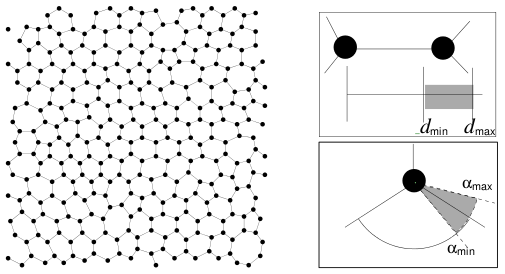
\includegraphics[width=0.4\textwidth]{Figures/amorphousSilicon.png}
	\caption{An amorphous solid under simulation.  A maximum vertex number of 3 is defined, along with minimum and maximum angles and bond lengths.  The goal is to find the minimum energy bond configuration. Taken from: Ref. \protect\citenum{Peinado1997gwt}}
	\label{fig:amorphousSilicon}
\end{figure}

\section{Simulated Annealing}
Simulated annealing is a stochastic approach towards minimizing the energy of a system.  It is related to Metropolis Monte Carlo and is based on the annealing of crystals, where a material is heated and then slowly cooled to allow for the formation of a crystal lattice.

\section{Genetic Algorithms}
Genetic Algorithms are probabilistic search algorithms based on natural selection~\cite{whitley_genetic_1994}.  In nature, the fittest individuals are most likely to survive and mate, and their offspring are expected to be healthier.  The algorithm represents the search space of the problem as a collection of individuals represented by character strings.  The algorithm randomly choses an initial population, and determines the fitness of each individual in this population.  Parents are then chosen from this population, and are combined to produce children.  From newly created individuals, a small number are chosen for mutation, i.e. their character string (genetic makeup) is changed at a randomly chosen mutation point.  The individuals with least fitness are removed from the population after each iteration to reduce the population to its initial size.  This new generation is then used in the next iteration and the process is repeated until stopping criteria are reached.

\section{Ant Colony Optimization}
Ant Colony Optimization~\cite{Dorigo96theant} draws inspiration from the behavior of ants as they develop a path from their nest to a food source.  As ants travel, they deposit pheromones.  These pheromones can be detected by other ants and the ants are more likely to follow a path with higher pheromone concentration.  In addition to the ants depositing pheromones, these pheromones will evaporate over time.  This means that shorter paths will allow larger pheromone concentrations to buildup as ants will be depositing pheromones quicker than they evaporate.  Eventually, the system will converge on a minimum solution.

\section{Go with the Winner Approaches}
Simulated annealing converges at a rate of $O(\frac{1}{n})$, where $n$ is the number of independent runs.  Using heuristic schemes such as the ``Go with the Winner (GWW),'' one can improve this convergence rate to $O(log \frac{1}{n})$ and have recently found their way into molecular modeling applications~\cite{Peinado1997gwt}.  In general terms, the GWW algorithm mirrors that of simulated annealing; however, each independent run is periodically reassessed to determine if one is converging upon a losing solution.  Runs that are deemed unlikely to succeed are immediately discarded while runs with a better chance of finding an optimal solution are replicated; thus, GWW generates an ensemble of independent runs filled with  ``winners.''

\section{Analysis}
We will study the minimization of surface reconstruction mapped onto the TSP.  Given that the deposition pattern of particles is not unique, all of the optimization schemes will need to generate an ensemble of possible models.  To investigate the configuration space coverage of these optimization schemes, we will initially start from known particle configurations, such as a hexagonal lattice, generate multiple optimization trajectories, and then analyze the solutions produced by each method.

Additionally, we will test the computational effort involved in each optimization scheme, focusing on the wall-clock time and the number of algorithm iterations/replicates are needed to generate an acceptable solution.  If time permits, we will also formulate these schemes into a parallel computing framework to improve their calculation efficiency.


\makeatletter
\newcommand{\adjustmybblparameters}{\setlength{\itemsep}{0ex}\setlength{\parsep}{0pt}}
\let\ORIGINALlatex@openbib@code=\@openbib@code
\renewcommand{\@openbib@code}{\ORIGINALlatex@openbib@code\adjustmybblparameters}
\makeatother

\bibliographystyle{unsrt}
\bibliography{AtomicScaleProposal}
\end{document}
